\chapter{Metodología de trabajo}
\label{chap:Metodologia de trabajo}
\Abstract{Para poder desarrollar w innovar es necesario primero definir una estructura base sobre la que edificar. Y se debe determinar un plan a seguir que sirva de guía.}

\section{Arquitectura del sistema}
\label{chap:Introducción sec:Arquitectura}
El sistema se compone de tres elementos claves: un robot industrial para poder interactuar con las piezas, una cámara RGB-D para la captura de imágenes y Python para el procesamiento de las imágenes y la toma de decisiones. Es necesario que estos tres elementos funcionen correctamente y estén comunicados entre sí. La arquitectura básica se puede ver en \autoref{chap:Introducción fig:Arq1}

\begin{figure}[h]
	\centering
	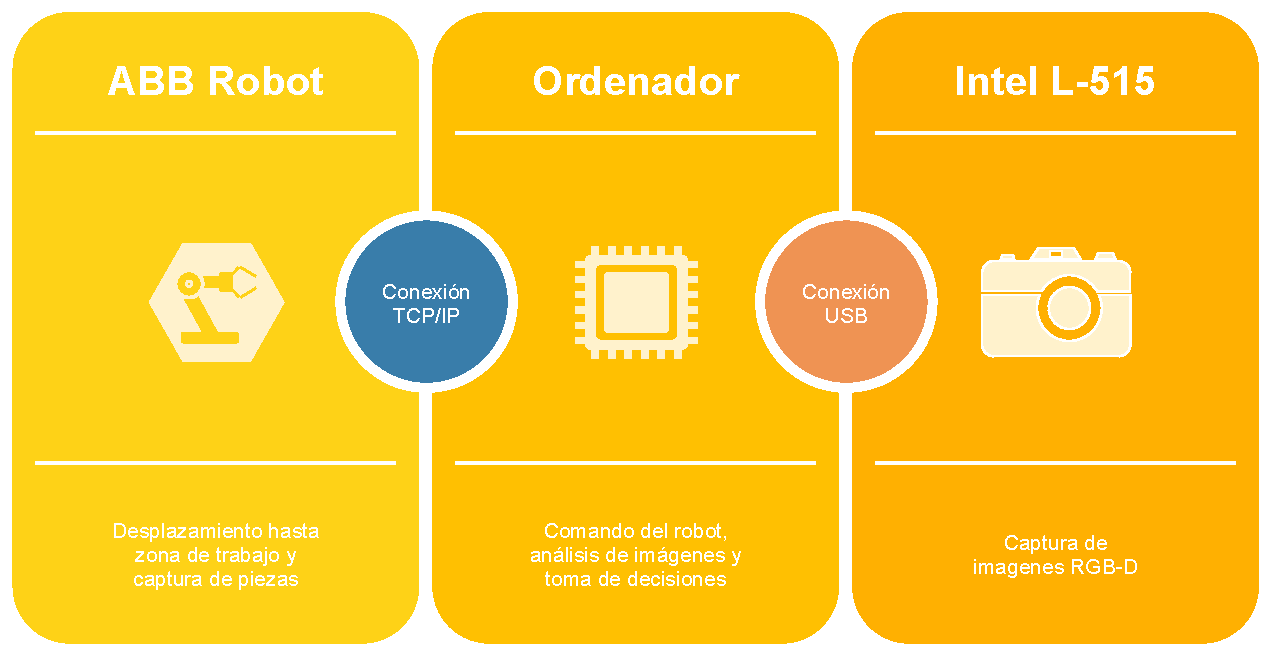
\includegraphics[width=0.9\textwidth]{Introduccion/Arquitectura.pdf}
	\caption{Esquema de la arquitectura del sistema}
	\label{chap:Introducción fig:Arq1}
	\vspace{-5pt}
\end{figure}

A continuación, se va a detallar todo el proceso desde el arranque del sistema hasta el final del mismo y se analizarán cada una de las etapas que constituyen el proceso. Este se puede ver gráficamente en \autoref{chap:Introducción fig:Arq2}. El sistema debe compenetrase con los sistemas actuales los cuales diseñan los pedidos que se deben de preparar y ensamblar. Estos pedidos se reciben y se procesan para establecer qué piezas se desean y en que orden deben de ser recogidas por medio de un proceso cíclico.

Una vez procesado el pedido y establecida la primera pieza a recoger se debe de desplazar el robot a la zona de trabajo y prepararse  para la captura de dicha pieza. Una vez reubicado el robot, un sistema de cámaras capturará la escena para determinar la posición de la pieza/piezas que se desean capturar frente a la posición del robot. Esta imagen es analizada por el sistema de visión artificial que se encargará de "en primera instancia" identificar las piezas para entre ellas poder centrarse solo en las que se desea capturar. A continuación, si se trata de una pieza de dimensiones grandes se analizará más en profundidad para determinar los posibles puntos de agarre. Y una vez determinados estos puntos de agarre un regresor determinará el centro exacto de dichos puntos de agarre así como el vector normal a dicho punto (dirección que debe emplear la muñeca del robot para capturar la pieza). Si por el contrario se trata de una pieza de dimensiones reducida se empleará el centro de la pieza como punto de agarre.

Esta información es transmitida al robot permitiéndole así poder capturar la pieza y depositarla en la cesta del pedido. Para ello este se deberá aproximar a la pieza seleccionada siguiendo en la medida de lo posible la trayectoria normal determinada. Al aproximarse a la pieza también deberá reducir la velocidad de operación para evitar colisionar.

\begin{figure}[ht]
	\centering
	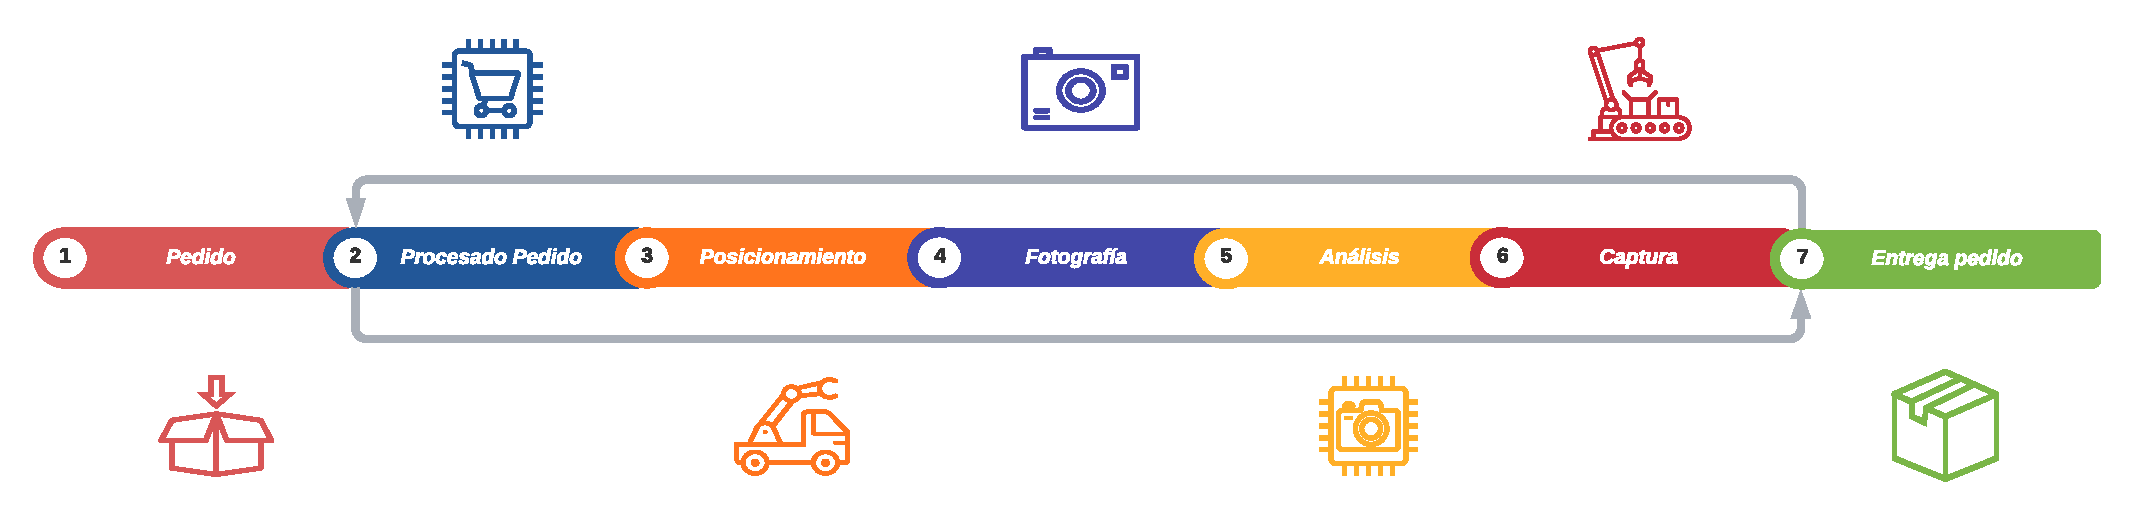
\includegraphics[width=1\textwidth]{Introduccion/Esquema arquitectura.pdf}
	\caption{Diagrama de las etapas del sistema}
	\label{chap:Introducción fig:Arq2}
	\vspace{-5pt}
\end{figure}

\section{Herramientas}
\label{chap:Introduccion sec:Herramientas}
\begin{itemize}
	\item Cámara Intel RealSense L515 \cite{IntelL515} y Wrapper de Python para Intel Realsense \cite{SDK}.
	\item Ordenador con los siguientes SO/paquetes/programas:
		\begin{itemize}
			\item Ubuntu 20.04 LTS
			\item Blender 2.93.5
			\item BlenderProc 2.0 (Blender API)
			\item PyTorch 1.10.1
			\item Tensorflow 2.7.0
			\item CUDAToolkit
			\item Python 3.8 o superior
			\item Conda ó miniconda
		\end{itemize}
\end{itemize}

\section{Cronograma}
\label{chap:Introducción sec:Cronograma}
La planificación del proyecto permite establecer un orden a seguir. No solo da estructura al proyecto, también ayuda a los desarrolladores a estructurar sus ideas. Es por ello que es vital y necesario establecer guías, objetivos e hitos a seguir.

\begin{table}[htbp]
  \centering
  \caption{Cronograma del proyecto}
    \begin{tabular}{p{16.5em}cccc}
    \rowcolor[rgb]{ .251,  .251,  .251} \multicolumn{1}{c}{\textcolor[rgb]{ 1,  1,  1}{\textbf{Descripción del hito}}} & \multicolumn{1}{c}{\textcolor[rgb]{ 1,  1,  1}{\textbf{Categoría}}} & \multicolumn{1}{c}{\textcolor[rgb]{ 1,  1,  1}{\textbf{Progreso}}} & \multicolumn{1}{c}{\textcolor[rgb]{ 1,  1,  1}{\textbf{Inicio}}} & \multicolumn{1}{c}{\textcolor[rgb]{ 1,  1,  1}{\textbf{Días}}} \\
    \rowcolor[rgb]{ .949,  .949,  .949} \textbf{MVP} &       &       &       &  \\
    Estado de la Cuestión & Hito  & 100\% & 01/06/2021 & 14  \\
    \rowcolor[rgb]{ .949,  .949,  .949} Base de datos sintéticas v0.1 & Objetivo & 100\% & 15/06/2021 & 14  \\
    Detección puntos de agarre & Hito  & 100\% & 29/06/2021 & 7  \\
    \rowcolor[rgb]{ .949,  .949,  .949} Driver Intel RealSense v0.1 & Objetivo & 100\% & 06/07/2021 & 7  \\
    Regresor - Tensorflow v0.1 & Objetivo & 100\% & 13/07/2021 & 7  \\
    \rowcolor[rgb]{ .949,  .949,  .949} Evaluación regresor & Objetivo & 100\% & 20/07/2021 & 3  \\
    \textbf{Base de datos sintética v1.0} &       &       &       &  \\
    \rowcolor[rgb]{ .949,  .949,  .949} Introducción de Arucos & Objetivo & 100\% & 01/09/2021 & 21  \\
    Extracción y lectura de normales & Hito  & 100\% & 22/09/2021 & 7  \\
    \rowcolor[rgb]{ .949,  .949,  .949} Preparación de bases de datos & Objetivo & 100\% & 29/09/2021 & 21  \\
    Actualización a Blenderproc 2.0 & Hito  & 100\% & 20/10/2021 & 7  \\
    \rowcolor[rgb]{ .949,  .949,  .949} Replicabilidad & Objetivo & 100\% & 27/10/2021 & 7  \\
    Riqueza de escenarios& Hito  & 15\% & 03/11/2021 & 14  \\
    \rowcolor[rgb]{ .949,  .949,  .949} Generación de base de datos real & Objetivo & 0\% & 17/11/2021 & 7  \\
    \textbf{Visión artificial v1.0} &       &       &       &  \\
    \rowcolor[rgb]{ .949,  .949,  .949} Estado de la Cuestión & Hito  & 100\% & 01/12/2021 & 10  \\
    Arquitectura del sistema & Objetivo & 100\% & 11/12/2021 & 14  \\
    \rowcolor[rgb]{ .949,  .949,  .949} YOLO & Objetivo & 100\% & 25/12/2021 & 7  \\
    TINY YOLO & Objetivo & 100\% & 01/01/2022 & 7  \\
    \rowcolor[rgb]{ .949,  .949,  .949} Regresor & Objetivo & 15\% & 08/01/2022 & 30  \\
    \textbf{Evaluación} &       &       &       &  \\
    \rowcolor[rgb]{ .949,  .949,  .949} Tamaño del dataset sintético & Objetivo & 0\% & 14/02/2022 & 30  \\
    Comparativa con dataset real & Objetivo & 0\% & 16/03/2022 & 10  \\
    \rowcolor[rgb]{ .949,  .949,  .949} \textbf{Redacción} &       &       &       &  \\
    Anexo B & Objetivo & 100\% & 01/12/2021 & 20  \\
    \rowcolor[rgb]{ .949,  .949,  .949} Memoria & Objetivo & 15\% & 01/04/2022 & 50  \\
    \end{tabular}%
  \label{chap:Introducción tab:plan}%
\end{table}%

\begin{figure}[ht]
	\centering
	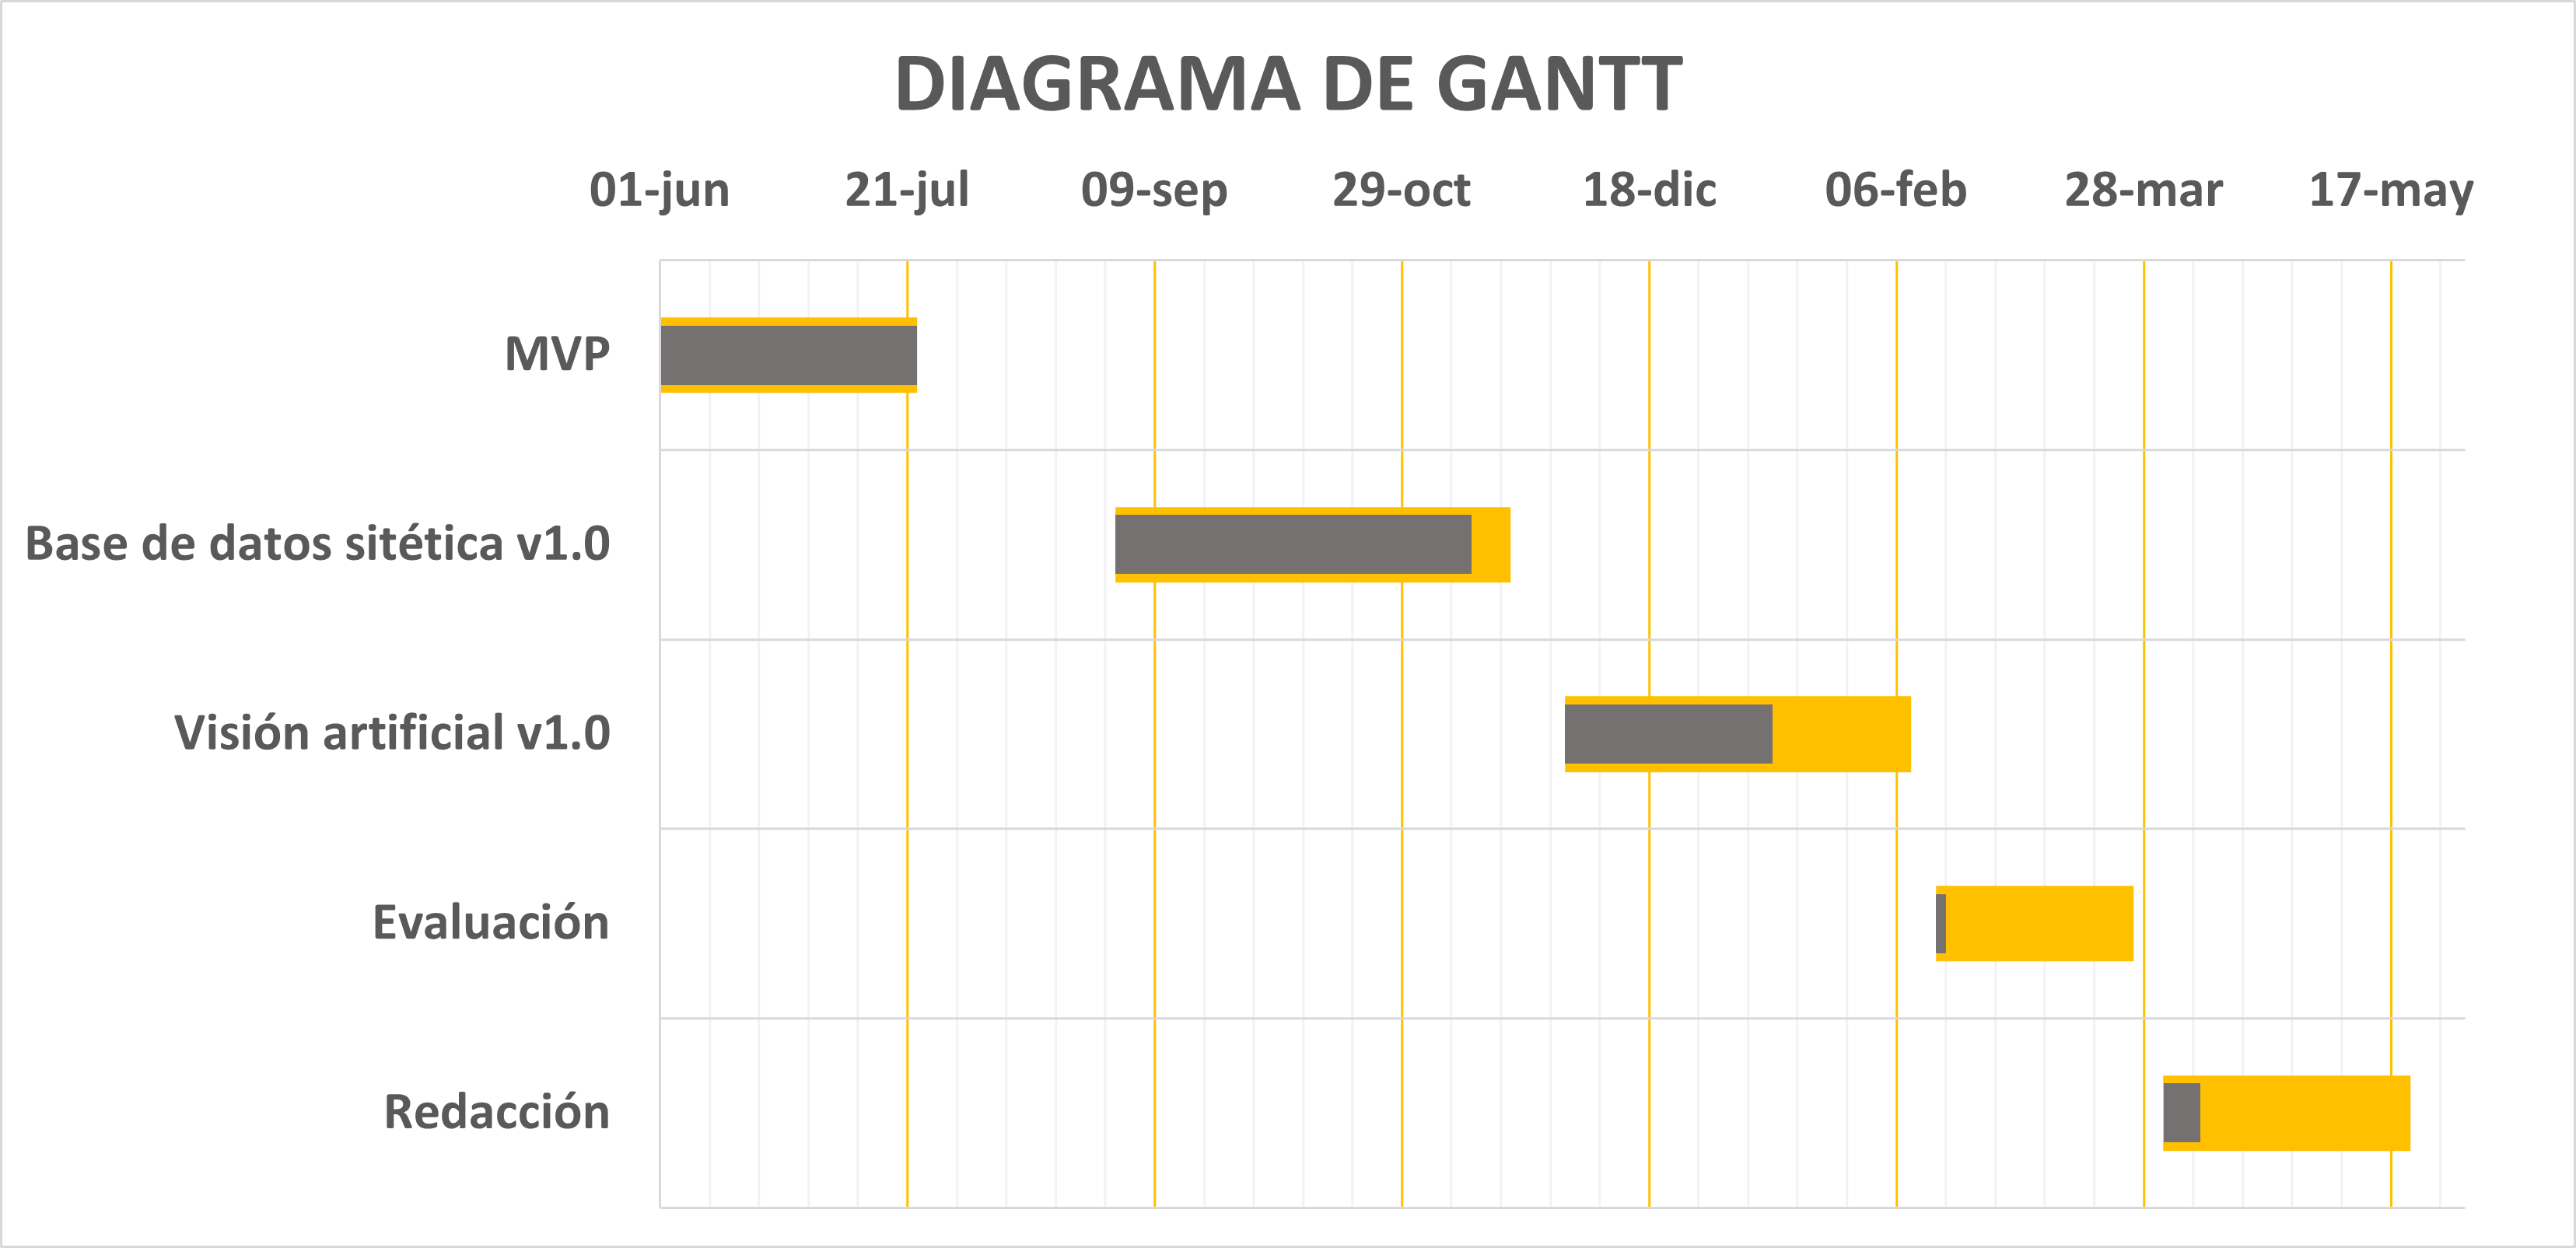
\includegraphics[width=0.8\textwidth]{Introduccion/Diagrama_de_gantt.png}
	\caption{Diagrama de gantt del proyecto}
	\label{chap:Introducción fig:Gantt}
	\vspace{-5pt}
\end{figure}